\documentclass[fleqn]{rbfin}

% The title should not exceed 10 words, while the abstract should be up to 150 words. 


%%%%%%%%%%%%%%%%%%%%%%%%%%%%%%%%%%%%
% COPYDESK INFO (DON'T WORRY ABOUT THESE)
%%%%%%%%%%%%%%%%%%%%%%%%%%%%%%%%%%%%

% Useless Watermark?
%\usepackage{draftwatermark}
%\SetWatermarkAngle{45}
%\SetWatermarkLightness{.92}
%\SetWatermarkFontSize{20pt}
%\SetWatermarkScale{6}
%\SetWatermarkText{\sf{Manuscript}}

\def\rbfinsubmitted{March 23, 2026}
% \def\rbfinaccepted{June 9, 2024}
\def\rbfinpublished{March 31, 2026}
\def\rbfineditor{Mr.\ Editor}
\def\rbfinDOI{10.xxxx/xxxx}

\def\rbfinyear{2025}
\def\rbfinvolume{24}
\def\rbfinpages{e202601}
\pagina{1}
%%%%%%%%%%%%%%%%%%%%%%%%%%%%%%%%%%%%

%%%%%%%%%%%%%%%%%%%%%%%%%%%%%%%%%%%%
% CUSTOM PACKAGES
% (LOAD CUSTOM PACKAGES BELOW)
%%%%%%%%%%%%%%%%%%%%%%%%%%%%%%%%%%%%
% \usepackage{tikz}

%%%%%%%%%%%%%%%%%%%%%%%%%%%%%%%%%%%%
% BEGIN DOCUMENT
%%%%%%%%%%%%%%%%%%%%%%%%%%%%%%%%%%%%
\begin{document}
% SELECT ARTICLE LANGUAGE
% Para artigos em PORTUGUÊS, alterar a linha abaixo para 
\selectlanguage{brazilian}
%\selectlanguage{english}
\frenchspacing

%%%%%%%%%%%%%%%%%%%%%%%%%%%%%%%%%%%%
% FRONT MATTER
%%%%%%%%%%%%%%%%%%%%%%%%%%%%%%%%%%%%
% ARTICLE TITLE
\title{Captura de Ineficiências Microestruturais na Curva DI usando PCA}
%\title{Arbitragem Estatística em Swaps DI: Capturando Anomalias da Curva} % Appears on title page

% ARTICLE SHORT TITLE
\shorttitle{\textit{Captura de Ineficiências Microestruturais na Curva DI usando PCA}} % appears on header every other page

%%%%%%%%%%%%%%%%%%%%%%%%%%%%%%%%%%%%
% AUTHOR INFORMATION
%%%%%%%%%%%%%%%%%%%%%%%%%%%%%%%%%%%%
\author{\centering
% Define institutions
\affiliations{1}{Fundação Getúlio Vargas, Escola de Matemática Aplicada, Rio de Janeiro, RJ}
%\affiliations{2}{Real Institute of Research}
% AUTHOR 1
\textbf{Adrian Castro}%
\email{adrianfilipe1@outlook.com}
\affiliationlink{1} % Match with the affiliations defined above
\orcidlink{0000-0000-0000}
\and % separate authors with \and
% AUTHOR 2
\textbf{Iara Castro}%
\email{iaramescuacastro@gmail.com}
\affiliationlink{1} % Match with the affiliations defined above
\orcidlink{0000-0000-0000}
\\[11pt]
% Print the affiliations:
\affiliationname{1}
}

%\and
% AUTHOR 3
%\textbf{Author Three}%
%\email{author.three@email}
%\affiliationlink{1} % Match with the affiliations defined above
%\affiliationlink{2} % Match with the affiliations defined above
%\orcidlink{0000-0000-0000}
% AND SO ON...

%\keywordslist{Curva DI; Swaps; Marcação a mercado; Risco de modelo; Engenharia financeira.}

\autor{Castro et al., \rbfinyear} % appears on header every other page
\autorlong{Castro, Adrian. \& Castro, Iara. (\rbfinyear{})} % only affects the “how-to-cite” text.
\maketitle

% ABSTRACT, KEYWORDS AND JEL
\begin{abstract}
	O mercado de juros futuros (DI) apresenta distorções geradas por fluxo de ordens. Este artigo propõe uma estratégia de arbitragem estatística do ruído microestrutural da curva DI (2021-2026), interpolada via \textit{Flat Forward} 252. Aplicamos a Análise de Componentes Principais (PCA) para neutralizar a dinâmica macroeconómica, operando a reversão à média do resíduo estocástico via \textit{z-score} (60 dias). No período \textit{out-of-sample} (2025-2026), os resultados evidenciam forte dependência espacial: a aplicação generalizada falha devido à não-estacionariedade nas pontas, mas nota-se altamente rentável na região central da curva. Utilizando o vértice M20 como estudo de caso, o modelo confirmou a captura da anomalia, gerando lucro absoluto, \textit{payoff} assimétrico e resiliência em testes de robustez. Conclui-se que a estratégia extrai \textit{alpha} descorrelacionado, mantendo o portefólio protegido do risco direcional da taxa Selic.
	
	\textbf{Palavras-chave:} Curvas DI; Arbitragem estatística; PCA; Reversão à média; DI1. \\
	\textbf{Códigos JEL:} G12; G13; C63.
\end{abstract}

%%%%%%%%%%%%%%%%%%%%%%%%%%%%%%%%%%%%
% END OF FRONT MATTER
%%%%%%%%%%%%%%%%%%%%%%%%%%%%%%%%%%%%

%%%%%%%%%%%%%%%%%%%%%%%%%%%%%%%%%%%%
% DOCUMENT MAIN SECTIONS
%%%%%%%%%%%%%%%%%%%%%%%%%%%%%%%%%%%%

\section{Introdução}\label{sec-intro}

A curva de juros é um dos principais objetos do mercado financeiro brasileiro, servindo de base para o apreçamento de ativos, a gestão de risco e a formulação de estratégias de hedge. No segmento de juros nominais, sua extração é fortemente ancorada nos contratos futuros de Depósito Interfinanceiro de um dia (DI1), negociados na B3, enquanto operações como swaps Pré x DI compõem o contexto institucional em que essa curva é utilizada para avaliação, proteção e arbitragem relativa.

Embora a modelagem tradicional trate a estrutura a termo como um objeto continuamente ajustado e sem fricções estáticas evidentes, a dinâmica observada em mercado é mais irregular. Choques transitórios de liquidez, rolagens de carteira, desequilíbrios temporários de oferta e demanda e fluxos institucionais concentrados podem provocar desalinhamentos localizados entre vértices da curva. Tais desvios, quando não associados a mudanças permanentes de regime, podem se manifestar como distorções estatisticamente mensuráveis.

%Tradicionalmente, a academia e os modelos de apreçamento assumem um mercado contínuo e livre de fricções, onde a curva se ajusta de maneira perfeitamente eficiente e sem arbitragem estática evidente. No entanto, a dinâmica real do mercado evidencia que fatores microestruturais como choques temporários de liquidez, fluxos de caixa institucionais assimétricos e rolagens de carteira, frequentemente provocam descolamentos pontuais em vértices específicos da curva. Essas ineficiências temporárias geram oportunidades para estratégias quantitativas que buscam explorar o prêmio de retorno à normalidade. 

Nesse contexto, este artigo tem como objetivo desenvolver e testar um modelo de arbitragem estatística aplicado aos derivativos de juros no Brasil. A proposta se aproxima da literatura de arbitragem estatística baseada em fatores e resíduos, na qual desvios em relação a uma estrutura sistemática são tratados como potenciais oportunidades de convergência \cite{avellaneda2010statistical}. Para isso, a curva DI é construída a partir dos vencimentos líquidos de DI1 e padronizada em maturidades constantes, de modo a permitir comparabilidade temporal entre os vértices. Sua dinâmica é então decomposta por meio da Análise de Componentes Principais (PCA), extraindo os fatores latentes associados a nível, inclinação e curvatura.


%Ao isolar o comportamento macroeconômico da curva, é possível identificar as anomalias de precificação nos vértices, tratadas aqui como resíduos. 

O componente não explicado pelos fatores principais é tratado como resíduo de precificação relativa e modelado através de um processo estocástico de reversão à média de Ornstein-Uhlenbeck, permitindo a geração de sinais matemáticos objetivos para a montagem de posições compradas e vendidas. Em primeiro lugar, o trabalho propõe uma estrutura empírica coerente com a microestrutura do mercado brasileiro de juros, centrada em DI1 e em dados públicos da B3. Em segundo lugar, testa se tais resíduos carregam conteúdo econômico suficiente para sustentar uma estratégia de arbitragem estatística após a consideração de custos operacionais e regras de execução.


\section{Contexto Institucional e Referencial Teórico}

\subsection{A Estrutura a Termo da Taxa de Juros (ETTJ) e a Dinâmica do Mercado DI}
A construção da Estrutura a Termo da Taxa de Juros (ETTJ) no mercado brasileiro baseia-se primordialmente nos contratos futuros de Depósito Interfinanceiro (DI1) negociados na B3, cujas convenções operacionais e de mercado são descritas nos manuais da própria infraestrutura de negociação \cite{b3manual}. Esses instrumentos refletem a expectativa do mercado para a taxa média do CDI over em diferentes horizontes temporais, sendo a principal referência para o apreçamento de ativos de renda fixa e derivativos de balcão.

O processo quantitativo de modelagem da curva inicia-se com a extração da taxa de juros implícita em cada contrato disponível (vértices da curva). A conversão do preço de mercado do contrato futuro para a taxa efetiva anualizada segue a convenção brasileira de contagem de prazos, estritamente baseada em 252 dias úteis, dada pela seguinte relação:

$$i = 100 \cdot \left[ \left( \frac{100.000}{PO} \right)^{\frac{252}{n}} - 1 \right]$$

onde $i$ representa a taxa de juros efetiva anualizada, $PO$ é o preço teórico ou de mercado do contrato futuro, e $n$ denota o número de dias úteis (NDU) exatos entre a data de cálculo e o vencimento do contrato.




\subsection{PCA como modelo principal de decomposição da curva}

A Análise de Componentes Principais (PCA) é o modelo empírico central deste estudo. Trata-se de uma ferramenta estatística amplamente utilizada na literatura financeira para identificar os fatores latentes que explicam a dinâmica da estrutura a termo das taxas de juros. Em aplicações sobre curvas de renda fixa, a evidência empírica demonstra que os três primeiros componentes principais são suficientes para explicar a maior parte (frequentemente mais de 97\% a 98\%) da variância total, permitindo uma representação parsimoniosa dos movimentos da curva ao longo do tempo \cite{litterman1991common}. \\ 

A literatura decompõe esses componentes nos seguintes fatores latentes:

\begin{itemize}
    \item \textbf{Nível}:
    %(Level / Parallel Shift)
    O primeiro fator explica a maior parte da variação do mercado (geralmente entre 85\% e 91\%) e corresponde a um deslocamento quase paralelo de todas as taxas da curva de juros. \\ 

    \item \textbf{Inclinação}:
    %(Slope / Twist)
    O segundo fator, que explica cerca de 8\% a 9\% da variância, reflete a mudança de inclinação da curva, indicando um movimento em que as taxas de curto prazo se movem em direção oposta às de longo prazo. \\ 

    \item \textbf{Curvatura}:
    %(Curvature / Bowing)
    O terceiro fator explica uma fração menor da variância (menos de 5\%) e representa o abaulamento da curva, onde as taxas curtas e longas se movem em uma direção.
    
\end{itemize}

%Para capturar analiticamente essa dinâmica impulsionada pelos componentes do PCA, o modelo paramétrico de Nelson-Siegel (1987) é amplamente adotado e modela a taxa à vista $R$ para uma maturidade $\tau$ através da seguinte equação:

%$$R(\tau) = \beta_0 + \beta_1 \left( \frac{1 - e^{-\tau/\lambda}}{\tau/\lambda} \right) + \beta_2 \left( \frac{1 - e^{-\tau/\lambda}}{\tau/\lambda} - e^{-\tau/\lambda} \right)$$

%Onde:

%\textit{$\beta_0$}: representa o Nível, pois o limite matemático quando $\tau \to \infty$ da função é o próprio $\beta_0$ (taxa de longo prazo). 
 
%\textit{$\beta_1$}: representa a Inclinação, carregando um peso que decai de 1 (quando $\tau \to 0$) para 0. Assim, a taxa de curtíssimo prazo é igual a $\beta_0 + \beta_1$. 

%\textit{$\beta_2$}:  representa a Curvatura, sendo acompanhado por uma função que inicia em 0, aumenta no médio prazo (formando a "corcunda") e decai a 0 no longo prazo. 

%\textit{$\lambda$}: é uma constante de decaimento que define onde o fator de curvatura atinge o seu máximo. Extensões como a de  \cite{svensson1994estimating} adicionam um quarto termo $\beta_3$ com um parâmetro de decaimento separado para modelar uma segunda corcunda na curva. \\

No presente artigo, o PCA é utilizado para separar a componente sistemática da curva DI da parcela idiossincrática não explicada pelos fatores comuns. Essa escolha permite modelar os desalinhamentos relativos entre vértices sem impor, a priori, uma estrutura paramétrica rígida à curva.

Essa interpretação fatorial dialoga com a literatura clássica de modelagem paramétrica da estrutura a termo. Em particular, o modelo de \cite{nelson1987parsimonious} representa a curva de juros por meio de parâmetros associados a nível, inclinação e curvatura onde modelam a taxa à vista para uma maturidade com um modelo-paramétrico, enquanto a extensão de \cite{svensson1994estimating} amplia a flexibilidade da parametrização ao adicionar um segundo termo de curvatura. De forma complementar, \cite{diebold2006forecasting} reforçam a interpretação econômica desses fatores em um contexto dinâmico, e \cite{wilmott2013paul} oferecem uma discussão aplicada sobre o uso de PCA e modelagem quantitativa em finanças. A interpretação econômica dos fatores de nível, inclinação e curvatura também é reforçada pela literatura dinâmica da curva de juros, notadamente em \cite{diebold2006forecasting}.

Neste estudo, contudo, Nelson-Siegel e Svensson são utilizados apenas como referências conceituais. O modelo efetivamente empregado para decompor a curva e gerar os resíduos operacionais é o PCA, por sua aderência direta à estrutura empírica dos dados e à proposta de arbitragem estatística baseada em fatores e resíduos. 


\subsection{Arbitragem Estatística e Reversão à Média}
Em estratégias de valor relativo, a hipótese central é que desvios extremos em relação a um padrão de equilíbrio tendem, ao menos parcialmente, a convergir ao longo do tempo. Neste artigo, essa ideia é aplicada ao resíduo da curva DI obtido após a remoção dos fatores comuns via PCA. Uma vez isolada a componente sistemática da curva, parte do resíduo remanescente pode refletir desalinhamentos temporários associados a liquidez, fluxo ou ruído microestrutural.

O alicerce matemático para esses modelos contínuos é o processo de Ornstein-Uhlenbeck, introduzido em finanças de forma seminal pelo modelo de \cite{vasicek1977equilibrium} para taxas de juros. A equação diferencial estocástica (SDE) do processo pode ser escrito como:

$$dr = a(b - r_t)dt + \sigma d W_t$$

em que $r_t$ representa a variável de interesse, $b$ é o nível de equilíbrio de longo prazo, $a>0$ é a velocidade de reversão à média, $\sigma$ é o parâmetro de volatilidade e $W_t$ é um processo de Wiener que possui média zero e variância igual a $dt$ ($d W_t = \epsilon \sqrt{dt}$).

No contexto deste estudo, a variável modelada é o resíduo estatístico extraído da curva. Assim, a utilidade do processo está menos na precificação estrutural de títulos e mais na interpretação dinâmica do desalinhamento observado. Quando o resíduo se afasta substancialmente de seu padrão recente, a hipótese de reversão sugere que esse desvio pode ser parcialmente corrigido ao longo do tempo, fornecendo base para a construção do sinal operacional.

Um parâmetro particularmente útil é a meia-vida do desvio, definida por: $t_{1/2} = \frac{\ln(2)}{a}$. A meia-vida fornece uma medida intuitiva do tempo esperado para que metade do desalinhamento seja absorvida, ajudando a calibrar o horizonte de carregamento da posição e a interpretar a persistência dos sinais. No desenho empírico deste artigo, essa lógica é operacionalizada por meio da normalização do resíduo com z-score em janela móvel, o que permite adaptar a identificação de anomalias ao regime recente de mercado.

A utilidade analítica desse modelo na apreçamento por arbitragem é que ele gera formulações affines (lineares) fechadas. Em sua formulação clássica, o processo também admite uma representação afim para o preço de ativos sensíveis à variável de estado, da forma $P(t, T) = A(t, T)e^{-B(t, T)r(t)}$ em que a sensibilidade temporal ao fator de risco é resumida por \(B(t,T)\). No caso do modelo com reversão à média, essa sensibilidade é amortecida ao longo do horizonte, sendo dada por \\ 

$$B(t, T) = \frac{1 - e^{-a(T-t)}}{a}$$

Isso significa que choques de curto prazo na variável (ou no resíduo do par cointegrado) não são precificados como persistentes no longo prazo, decaindo a uma taxa exponencial dependente de $a$, permitindo calcular qual seria o valor "justo" ou o "desalinhamento" explorado na arbitragem.

\subsection{Interpolação de Maturidade Constante (Flat Forward 252)}

Para a construção de uma curva de juros contínua e passível de modelagem via PCA, é imperativo mitigar o efeito de \textit{roll-down} (envelhecimento) dos contratos futuros. A literatura quantitativa recomenda a interpolação dos vértices observados em pontos de maturidade constante. Do ponto de vista metodológico, a literatura de construção de curvas destaca que a escolha do método de interpolação afeta a regularidade da estrutura a termo e a estabilidade das taxas implícitas \cite{hagan2006interpolation}. Para refletir com exatidão a microestrutura de apreçamento do mercado brasileiro, adota-se o método de Interpolação \textit{Flat Forward} 252, metodologia oficial da B3 para a Curva DI x Pré \cite{b3manual}. Este método garante que a taxa a termo permaneça constante entre os vértices observados. A taxa interpolada é dada pela equação:

\begin{equation}
i_{interp} = \left[ \left( \left( \frac{\left( 1 + \frac{L_{post}}{100} \right)^{\frac{DU_{post}}{252}}}{\left( 1 + \frac{L_{ant}}{100} \right)^{\frac{DU_{ant}}{252}}} \right)^{\frac{DU - DU_{ant}}{DU_{post} - DU_{ant}}} \times \left( 1 + \frac{L_{ant}}{100} \right)^{\frac{DU_{ant}}{252}} \right)^{\frac{252}{DU}} - 1 \right] \times 100
\label{eq:flat_forward}
\end{equation}

Em que $DU$ representa os dias úteis do vértice alvo, e os subscritos $ant$ e $post$ referem-se aos vértices observados imediatamente anterior e posterior.

\subsection{Estacionariedade Local e Z-Score Estocástico}

A premissa da arbitragem estatística é a reversão à média do resíduo não explicado pelo modelo fatorial (PCA). Contudo, em mercados emergentes, testes globais de estacionariedade frequentemente falham devido a quebras estruturais e mudanças abruptas no regime de política monetária. Para contornar essa limitação teórica, introduz-se o conceito de estacionariedade local. O gatilho de operação é normalizado através de um \textit{z-score} com janela móvel, definindo um prêmio de risco dinâmico:



$$Z_t = \frac{X_t - \mu_w}{\sigma_w}$$



Onde $X_t$ é o \textit{spread} residual no tempo $t$, $\mu_w$ é a média móvel do \textit{spread} e $\sigma_w$ é o desvio padrão na janela de $w$ dias. Essa abordagem assegura que o modelo identifique anomalias microestruturais em relação ao regime de mercado estritamente recente, ignorando distorções de longo prazo.

\section{Metodologia}

A arquitetura do modelo de arbitragem estatística proposto foi desenvolvida em ambiente Python, com uso de bibliotecas voltadas à manipulação de dados, álgebra linear e econometria de séries temporais.

%utilizando as bibliotecas pandas e numpy para manipulação matricial, scikit-learn para a extração de componentes principais e statsmodels para a testagem de estacionariedade.

A implementação divide-se em quatro blocos: (i) construção da base de dados; (ii) organização da curva DI em vértices comparáveis ao longo do tempo; (iii) decomposição por PCA e estimação dos resíduos; e (iv) estruturação do backtest com regras explícitas de execução.
%(iv) modelagem do processo estocástico e estruturação do backtest institucional.

\subsection{Coleta de Dados e Criação da Curva}

A base de dados é obtida diretamente dos boletins diários da B3 em formato XML. Extraímos os contratos de DI1 futuros e suas respectivas taxas e datas de vencimento.

%daí encontramos a taxa e calculamos o NDU com base nos feriados Brasileiros da ANBIMA

Após a ingestão dos arquivos, os contratos são filtrados para o universo de DI1 e alinhados por data de pregão e maturidade. Em seguida, calcula-se o número de dias úteis até o vencimento ($NDU$) com base em calendário compatível com o mercado local, incorporando fins de semana e feriados nacionais relevantes. Esse procedimento permite expressar cada observação em termos de prazo efetivo e taxa comparável, formando a malha temporal que sustenta as etapas seguintes da análise.

\subsection{Organização da Curva em Vértices}

Uma vez obtidos os contratos válidos para cada dia, a curva é representada por um conjunto de vértices observados associados aos vencimentos líquidos disponíveis. Quando necessário para comparabilidade entre datas, aplica-se o preenchimento dos intervalos entre vencimentos observados de forma consistente com a convenção adotada para a curva DI x Pré, preservando a estrutura temporal dos dados.

Como o objetivo do artigo é estudar resíduos de precificação relativa, a etapa de construção da curva tem papel preparatório. O foco da análise recai sobre a estabilidade da representação dos vértices ao longo do tempo, condição necessária para a aplicação do PCA e para a construção de séries históricas comparáveis.

Para viabilizar a análise matricial simétrica requerida pelo PCA, a curva diária de juros foi submetida à interpolação \textit{Flat Forward} 252 (conforme Equação \ref{eq:flat_forward}). Esse procedimento padronizou os dados em 36 vértices mensais fixos de maturidades constantes em múltiplos de 21 dias úteis (M1 a M36). Essa densidade garante a captura de microdistorções em toda a extensão da curva líquida.


\subsection{Decomposição Fatorial e Estimação dos Resíduos}

Com a curva organizada em formato matricial, aplica-se o PCA sobre a base histórica para extrair os fatores dominantes de variação. O número de componentes retidos é definido de modo a capturar a maior parte da variância total, preservando a interpretação econômica dos fatores principais.

A curva reconstruída a partir desses componentes define a parcela sistemática dos movimentos de juros. A diferença entre a observação efetiva e a reconstrução fornece os resíduos utilizados como insumo da estratégia. Esses resíduos podem ser analisados individualmente por vértice ou agregados em combinações lineares que representem relações de valor relativo ao longo da curva.

\subsection{Estruturação do Backtest Out-of-Sample}

Para mitigar o viés de antecipação (\textit{look-ahead bias}) e validar a robustez operacional do modelo, o algoritmo foi submetido a um teste cronológico de caminhada à frente (\textit{walk-forward}). O conjunto de dados foi dividido em dois períodos mutuamente excludentes:

\begin{itemize}
    \item \textbf{\textit{In-Sample} (Treinamento):} De janeiro de 2021 a dezembro de 2024. Período utilizado exclusivamente para a calibração do modelo PCA e extração dos fatores estruturais.
    \item \textbf{\textit{Out-of-Sample} (Teste Cego):} De janeiro de 2025 a fevereiro de 2026. Período no qual as cargas fatoriais (\textit{loadings}) foram fixadas, e a estratégia simulou a execução diária em dados não observados pelo modelo de treinamento.
\end{itemize}

O gatilho estocástico ($z-score$) foi calibrado com uma janela móvel de $w = 60$ dias úteis. As regras de execução (\textit{trading rules}) determinam a entrada (\textit{short} na taxa) quando $Z_t > 2$, assumindo superprecificação momentânea, e a entrada oposta (\textit{long} na taxa) quando $Z_t < -2$, assumindo subprecificação. A convergência da anomalia, definida pelo cruzamento $Z_t = 0$, aciona a liquidação da posição e a apuração do PnL (\textit{Profit and Loss}).


Por fim, com o objetivo de favorecer a transparência e a reprodutibilidade dos resultados, os códigos utilizados no processamento dos dados, na construção da curva DI em maturidade constante, na decomposição por PCA, na geração dos sinais estatísticos e na execução do backtest foram disponibilizados em repositório público. O material pode ser acessado em: \url{https://github.com/adrianfilipe/artigo_di}.


\section{Resultados}
\subsection{Análise Preliminar: A Falha da Aplicação Ingénua}

Antes de aprofundar a viabilidade operacional do modelo em segmentos específicos, é imperativo analisar o comportamento da estratégia numa aplicação "naive" (ingénua), simulando a execução simultânea das regras de \textit{trading} em todos os vértices operáveis da curva DI. Esta análise preliminar serve como um "caso base" para isolar os componentes estruturais do risco de mercado que o PCA não consegue neutralizar completamente em horizontes táticos. A Figura \ref{fig:pnl_geral} apresenta o PnL acumulado consolidado da carteira geral ao longo do período \textit{out-of-sample} (2025-2026), calculando a soma aritmética dos retornos diários de cada vértice operado sob os parâmetros base ($Z=2.0$ e $w=60$).

\begin{figure}[ht]
    \centering
    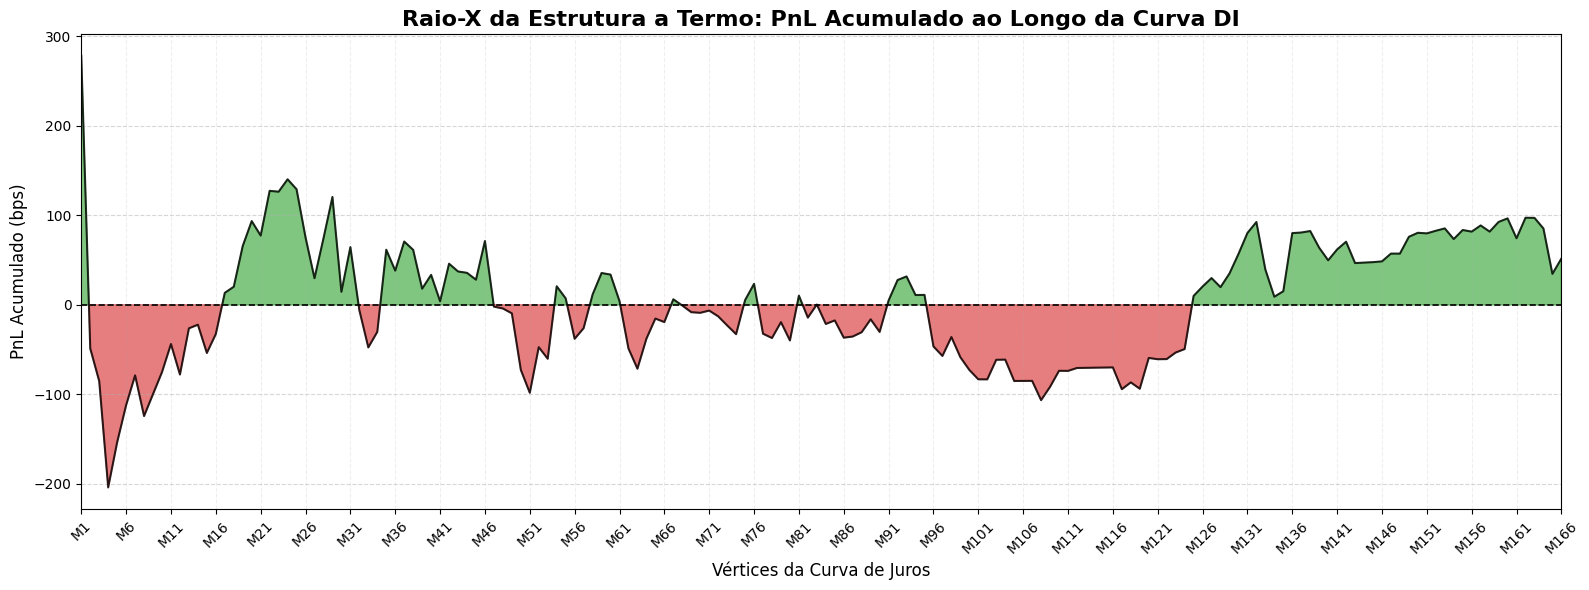
\includegraphics[width=\textwidth]{media/image.png} % Certifique-se de que este é o nome do ficheiro da imagem
    \caption{PnL Acumulado da Carteira Geral (Soma de Todos os Vértices) - \textit{Out-of-Sample} (2025-2026)}
    \label{fig:pnl_geral}
\end{figure}

A observação da Figura \ref{fig:pnl_geral} revela um cenário financeiramente catastrófico para a aplicação generalizada da estratégia. Nota-se um rebaixamento (\textit{drawdown}) súbito e agressivo logo no início de 2025, de onde a carteira nunca recupera, acumulando um prejuízo superior a 600 bps no final do teste cego. Este resultado, longe de invalidar a tese do artigo, constitui uma evidência empírica robusta sobre a microestrutura da curva DI brasileira. O colapso do PnL consolida a hipótese de que a premissa de reversão à média estatística ($StatArb$) não é universal. O modelo ingénuo ignora que o período de 2025 foi marcado por uma forte quebra de regime macroeconômico (início do ciclo de alta da Selic e aumento das preocupações fiscais). Sob estas condições, o resíduo estatístico do PCA em vértices específicos (notadamente na ponta curta controlada pelo Banco Central e na ponta longa dominada pelo risco fiscal) não representou ruído microestrutural reversível, mas sim um \textit{momentum} direcional persistente, que "engoliu" os lucros gerados nos vértices intermediários. Esta falha sistémica justifica a necessidade de decompor a curva e focar a análise em segmentos que apresentam estacionariedade local tática.

\subsection{A Dinâmica Fatorial da Curva DI}

A aplicação da Análise de Componentes Principais (PCA) sobre a matriz de covariância dos 36 vértices interpolados revelou uma elevada concentração da variância nos três primeiros fatores latentes, corroborando a literatura clássica de estrutura a termo. Conforme evidenciado na Tabela \ref{tab:variancia_pca}, o Fator 1 (Nível) explicou 93,4\% da dinâmica da curva, refletindo de forma predominante os choques paralelos de política monetária. O Fator 2 (Inclinação) representou 4,4\% da variância, enquanto o Fator 3 (Curvatura) capturou 1,1\%. 

Conjuntamente, os três componentes explicaram 98,9\% da movimentação estrutural da curva DI no período \textit{in-sample}, atestando a eficácia da interpolação \textit{Flat Forward} 252 na remoção de ruídos associados ao \textit{roll-down} dos contratos. Este altíssimo grau de explicação da parcela macroeconômica justifica estatisticamente o isolamento da variância não explicada — o resíduo exato de 1,1\% — como a representação pura do prêmio de liquidez e do ruído microestrutural, os quais constituem o alvo exploratório da estratégia de arbitragem.



\begin{table}[ht]
\centering
\caption{Variância explicada pelos componentes principais (período \textit{in-sample})}
\label{tab:variancia_pca}
\begin{tabular}{lcc}
\toprule
\textbf{Componente (Fator)} & \textbf{Variância (\%)} & \textbf{Acumulado (\%)} \\
\midrule
PC1 (Nível)       & 93,4 & 93,4 \\
PC2 (Inclinação)  & 4,4  & 97,8 \\
PC3 (Curvatura)   & 1,1  & 98,9 \\
\bottomrule
\end{tabular}
\end{table}

Como complemento à análise principal, os loadings completos dos três primeiros componentes principais ao longo dos vértices da curva são apresentados no Apêndice A. A Figura A1 permite visualizar, de forma mais detalhada, a sensibilidade de cada vértice aos fatores de nível, inclinação e curvatura, reforçando a interpretação econômica da decomposição fatorial adotada no artigo.



\subsection{Mapeamento das Ineficiências Microestruturais}
\begin{table}[H]
\centering
\caption{Reversão à média dos resíduos por vértice (estatísticas e meia-vida)}
\label{tab:reversao_media}
\begin{tabular}{lccc}
\toprule
\textbf{Vértice (Alvo)} & \textbf{Meia-vida (dias)} & \textbf{$\sigma$ (bps)} & \textbf{$\% (|Z| > 2)$} \\ 
\midrule
Curto (M6)              & 1119,80                   & 68,86                   & 16,51\%                 \\
Médio-Curto (M12)       & 140,82                    & 24,85                   & 13,08\%                 \\
Médio (M20)             & 183,86                    & 17,25                   & 11,04\%                 \\
Médio-Longo (M40)       & 60,32                     & 9,30                    & 11,90\%                 \\
Longo (M60)             & 21,66                     & 5,03                    & 12,33\%                 \\
Longo (M80)             & 9,52                      & 3,02                    & 10,93\%                 \\
Longo (M100)            & 46,63                     & 5,28                    & 12,33\%                 \\
Longo (M120)            & 71,04                     & 5,29                    & 12,33\%                 \\
Longo (M140)            & 15,03                     & 2,86                    & 12,22\%                 \\
Extremo Longo (M166)    & 36,83                     & 5,33                    & 15,54\%                 \\ 
\bottomrule
\end{tabular}
\floatfoot{Nota: Meia-vida extraída do coeficiente de reversão ($\theta$) da regressão OLS do modelo de Ornstein-Uhlenbeck. O desvio padrão ($\sigma$) e a frequência empírica de distorções extremas ($|Z| > 2$) referem-se à janela de \textit{in-sample}.}
\end{table}

A análise das estatísticas do processo de Ornstein-Uhlenbeck, sumarizadas na Tabela \ref{tab:reversao_media}, evidencia o comportamento heterogêneo do prêmio de risco ao longo da Estrutura a Termo da Taxa de Juros. Nota-se, primeiramente, a marcante não-estacionariedade da ponta curta da curva. O vértice M6, por exemplo, apresenta uma meia-vida de reversão excessivamente longa, superior a 1.110 dias, acompanhada da maior volatilidade residual de todo o espectro ($\sigma = 68,86$ bps). Este comportamento corrobora a hipótese de que a ponta curta está deterministicamente ancorada ao ciclo de política monetária traçado pelo Banco Central; logo, choques nestes vértices configuram mudanças persistentes de regime macroeconómico que não revertem à média, inviabilizando operações de valor relativo de curto prazo. Em contrapartida, à medida que a análise avança para o "miolo" da curva (vértices M12 a M40), observa-se um rápido decaimento assintótico tanto da meia-vida, que recua para o intervalo de 60 a 184 dias, quanto da volatilidade do resíduo, que se estabiliza entre 9 e 25 bps. É exatamente nesta região intermediária que a estratégia de arbitragem estatística encontra a sua janela de viabilidade ideal. A volatilidade latente é atrativa o suficiente para gerar distorções operáveis, enquanto a força de reversão à média — impulsionada pelo intenso fluxo de tesourarias e rolagens de \textit{hedge} institucional — atua com a rapidez necessária para garantir a convergência e o fecho das posições num horizonte tático.

Além da dependência espacial, os resultados revelam um comportamento leptocúrtico (\textit{fat tails}) intrínseco aos resíduos em toda a extensão da curva. Sob a premissa de uma distribuição normal, esperar-se-ia que o gatilho estocástico rompesse a barreira de $|Z| > 2$ em aproximadamente 4,5\% das observações. Contudo, a frequência empírica de distorções extremas oscila sistematicamente entre 11\% e 16,5\%. Esta evidência atesta que os desvios não explicados pela dinâmica fatorial do PCA não refletem meros erros gaussianos de estimação, mas sim anomalias microestruturais severas. Tratam-se de choques de liquidez, desequilíbrios momentâneos de oferta e procura e assimetrias de fluxo no livro de ordens, constituindo a proxy para desalinhamentos relativos do modelo proposto.

Uma visualização complementar da distribuição temporal e transversal das anomalias ao longo da curva é apresentada no Apêndice A. Em particular, a Figura A2 reporta o heatmap do z-score por vértice, permitindo identificar de forma mais clara a concentração das distorções em determinados trechos e períodos da amostra.




\subsection{Performance Operacional (O Backtest Cego)}

O \textit{backtest out-of-sample} demonstrou a exequibilidade operacional e a eficiência da estratégia na alocação de risco. Focando no vértice de médio prazo (M20), o modelo gerou um retorno absoluto acumulado de 93,56 bps ao longo do período de teste. Um ponto de destaque é a baixíssima correlação temporal com o risco direcional: dos 229 dias operacionais analisados, o algoritmo esteve posicionado no mercado durante apenas 107 dias (aproximadamente 46,7\% do tempo), permanecendo neutro e protegido nas restantes sessões. 

A Tabela \ref{tab:performance} resume os \textit{KPIs} (Key Performance Indicators) da estratégia. O modelo atingiu um pico de rentabilidade máxima (\textit{High Watermark}) de 106,89 bps, limitando o rebaixamento (\textit{Max Drawdown}) a -40,76 bps. Reitera-se o \textit{Payoff} assimétrico de 4,37, o qual evidencia que a regra estocástica de liquidação ($Z=0$) atua como um mecanismo de \textit{stop loss} altamente eficiente, estancando as perdas rapidamente enquanto maximiza a captura do prémio de liquidez nas operações vencedoras.

\begin{table}[H]
\centering
\caption{Métricas de performance do backtest (\textit{out-of-sample} - Vértice M20)}
\label{tab:performance}
\begin{tabular}{lc}
\toprule
\textbf{Métrica}             & \textbf{Resultado (Bruto)} \\ 
\midrule
Retorno Acumulado (PnL)      & 93,6 bps                  \\
Pico de Lucro (\textit{High Watermark}) & 106,9 bps      \\
Max Drawdown                 & -40,8 bps                 \\
Taxa de Acerto (Hit rate)    & 66,7\%                     \\
Payoff (Gain/Loss)           & 4,4                       \\
Nº de trades                 & 3                          \\
Dias posicionado no mercado  & 107 dias                   \\
Dias operacionais totais     & 229 dias                   \\
Taxa de Exposição ao Mercado & 46,7\%                     \\ 
\bottomrule
\end{tabular}
\end{table}

%Mostra se o resultado depende de “tuning” muito específico.
% Se só funciona com w = 60, Z=2, o avaliador pode suspeitar de overfitting.

\begin{table}[H]
\centering
\caption{Análise de Robustez: sensibilidade à janela móvel e limiar estocástico (\textit{out-of-sample} - M20)}
\label{tab:robustez}
\begin{tabular}{lcccc}
\toprule
\textbf{Configuração}                  & \textbf{PnL (bps)} & \textbf{Max DD (bps)} & \textbf{Hit Rate} & \textbf{Nº Trades} \\ 
\midrule
\textbf{$|Z| > 2.0 \ | \ w=60$ (Base)} & \textbf{93,6}      & \textbf{-40,8}        & \textbf{66,7\%}   & \textbf{3}         \\
$|Z| > 2.0 \ | \ w=40$                 & 128,6              & -36,5                 & 100,0\%           & 4                  \\
$|Z| > 2.0 \ | \ w=120$                & 56,0               & -44,3                 & 100,0\%           & 1                  \\
$|Z| > 1.5 \ | \ w=60$                 & 119,5              & -40,8                 & 75,0\%            & 4                  \\
$|Z| > 2.5 \ | \ w=60$                 & 56,6               & -36,5                 & 100,0\%           & 3                  \\ 
\bottomrule
\end{tabular}
\floatfoot{Nota: Todos os cenários alternativos apresentaram rentabilidade absoluta positiva e rebaixamentos (\textit{drawdowns}) controlados, refutando a hipótese de \textit{data snooping} ou \textit{overfitting} na calibração dos parâmetros base.}
\end{table}

Para afastar o risco de \textit{data snooping} e assegurar que a rentabilidade do modelo não é mero artefacto de uma otimização excessiva (\textit{overfitting}) dos hiperparâmetros, realizou-se uma análise de sensibilidade estática no período \textit{out-of-sample}, cujos resultados estão consolidados na Tabela \ref{tab:robustez}. A principal evidência de robustez estrutural reside no fato de que todas as permutações de parâmetros — tanto em diferentes horizontes de janela móvel ($w$) quanto em diferentes níveis de agressividade do gatilho estocástico ($Z$) — produziram um PnL acumulado estritamente positivo, acompanhado de rebaixamentos (Max Drawdowns) controlados.

Do ponto de vista da reatividade da média móvel, a redução da janela para $w=40$ dias elevou o retorno capturado para 128,6 bps e o \textit{Hit Rate} para 100\%, com a execução de uma operação adicional. Este resultado sugere que, em janelas de stresse microestrutural agudo, uma métrica de equilíbrio mais reativa pode capturar com maior precisão o prémio de liquidez antes da sua dissipação. Por outro lado, o alongamento da janela para $w=120$ dias suavizou excessivamente a referência de precificação, reduzindo o número de sinais a apenas um \textit{trade} e limitando a rentabilidade a 56,0 bps.

A análise do limiar de entrada corrobora o clássico \textit{trade-off} entre frequência operacional e qualidade do sinal na arbitragem estatística. A flexibilização do gatilho para $|Z| > 1.5$ aumentou a captação bruta de prémio (119,5 bps), mas incorreu numa maior captura de ruído e falsos rompimentos, penalizando o \textit{Hit Rate} (75,0\%). Em contrapartida, a imposição de uma barreira restritiva de $|Z| > 2.5$ operou como um filtro de anomalias extremas, garantindo uma taxa de acerto perfeita (100\%), embora sacrificando parte do custo de oportunidade (56,6 bps). No cômputo geral, a parametrização base ($w=60$ e $|Z|>2.0$) manteve-se como um ponto ótimo de ancoragem teórica, equilibrando assertividade, proteção contra \textit{drawdowns} e um fluxo operacional consistente.



\section{Considerações Finais}

Este artigo propôs e validou uma estrutura quantitativa para a extração de prémio de risco microestrutural na curva de juros brasileira (DI), isolando o ruído de liquidez através da Análise de Componentes Principais (PCA) e operando a sua reversão à média. Os resultados são consistentes com a hipótese de que parte da variância residual captura desalinhamentos relativos potencialmente exploráveis. No entanto, o estudo demonstrou que esta ineficiência não se distribui de forma homogénea ao longo da estrutura a termo. A aplicação generalizada da estratégia evidenciou que a ponta curta, rigidamente ancorada pela política monetária, e a ponta longa, dominada por prémios de risco fiscal persistentes, carecem da estacionariedade local necessária para suportar operações de valor relativo de curto prazo.

O grande contributo empírico deste trabalho reside no mapeamento do "miolo" da curva (particularmente na região do vértice M20) como o segmento ótimo para a arbitragem estatística. O rigoroso \textit{backtest out-of-sample} sugeriu que, nesta região de elevada liquidez e intenso fluxo de \textit{hedge} institucional, o modelo é capaz de identificar anomalias com precisão. A estratégia gerou um retorno absoluto robusto e um \textit{payoff} fortemente assimétrico, mantendo o portfólio com exposição nula ao risco direcional da taxa Selic durante mais de metade do ano operacional, provando o valor do gatilho estocástico de z-score como um mecanismo eficiente de controle de risco e alocação de capital.

Apesar da consistência dos resultados, o modelo apresenta limitações inerentes à sua formulação teórica que abrem caminho para pesquisas futuras. A simulação assumiu a execução das ordens aos preços de fecho diários, não incorporando os custos de transação explícitos (taxas da B3) nem a fricção implícita do \textit{bid-ask spread}, fatores que podem comprimir a rentabilidade líquida em cenários de estresse de liquidez. Para desenvolvimentos futuros, sugere-se a incorporação de modelos de \textit{Machine Learning} (como \textit{Reinforcement Learning}) para a calibração dinâmica da janela móvel e do limiar de ativação em função do regime de volatilidade intradiária. Adicionalmente, a replicação desta arquitetura na curva de juros reais (contratos DAP/Cupom IPCA) constituiria uma extensão natural e valiosa para a literatura de apreçamento de ativos em mercados emergentes.


\bibliography{references.bib}\label{refs}
\bibliographystyle{dcu-rbfin}


% APPENDIX
%%%%%%%%%%%%%%%%%%%%%%%%%%%%%%%%%%%%
\rbfinappendix
\section{Material complementar}

As figuras desta seção complementam os resultados apresentados no texto principal.

\begin{figure}[H]
	\centering
	
\includegraphics[width=0.95\linewidth]{media/pca_loadings.png}
	\caption{PCA da curva DI: loadings dos três primeiros componentes ao longo dos vértices da curva. Entre parênteses, reporta-se a variância explicada por cada componente. A figura complementa a Tabela 1 ao oferecer uma visualização detalhada da sensibilidade dos vértices aos fatores de nível, inclinação e curvatura.}
	\label{fig:apendice_loadings}
\end{figure}

\begin{figure}[H]
	\centering
	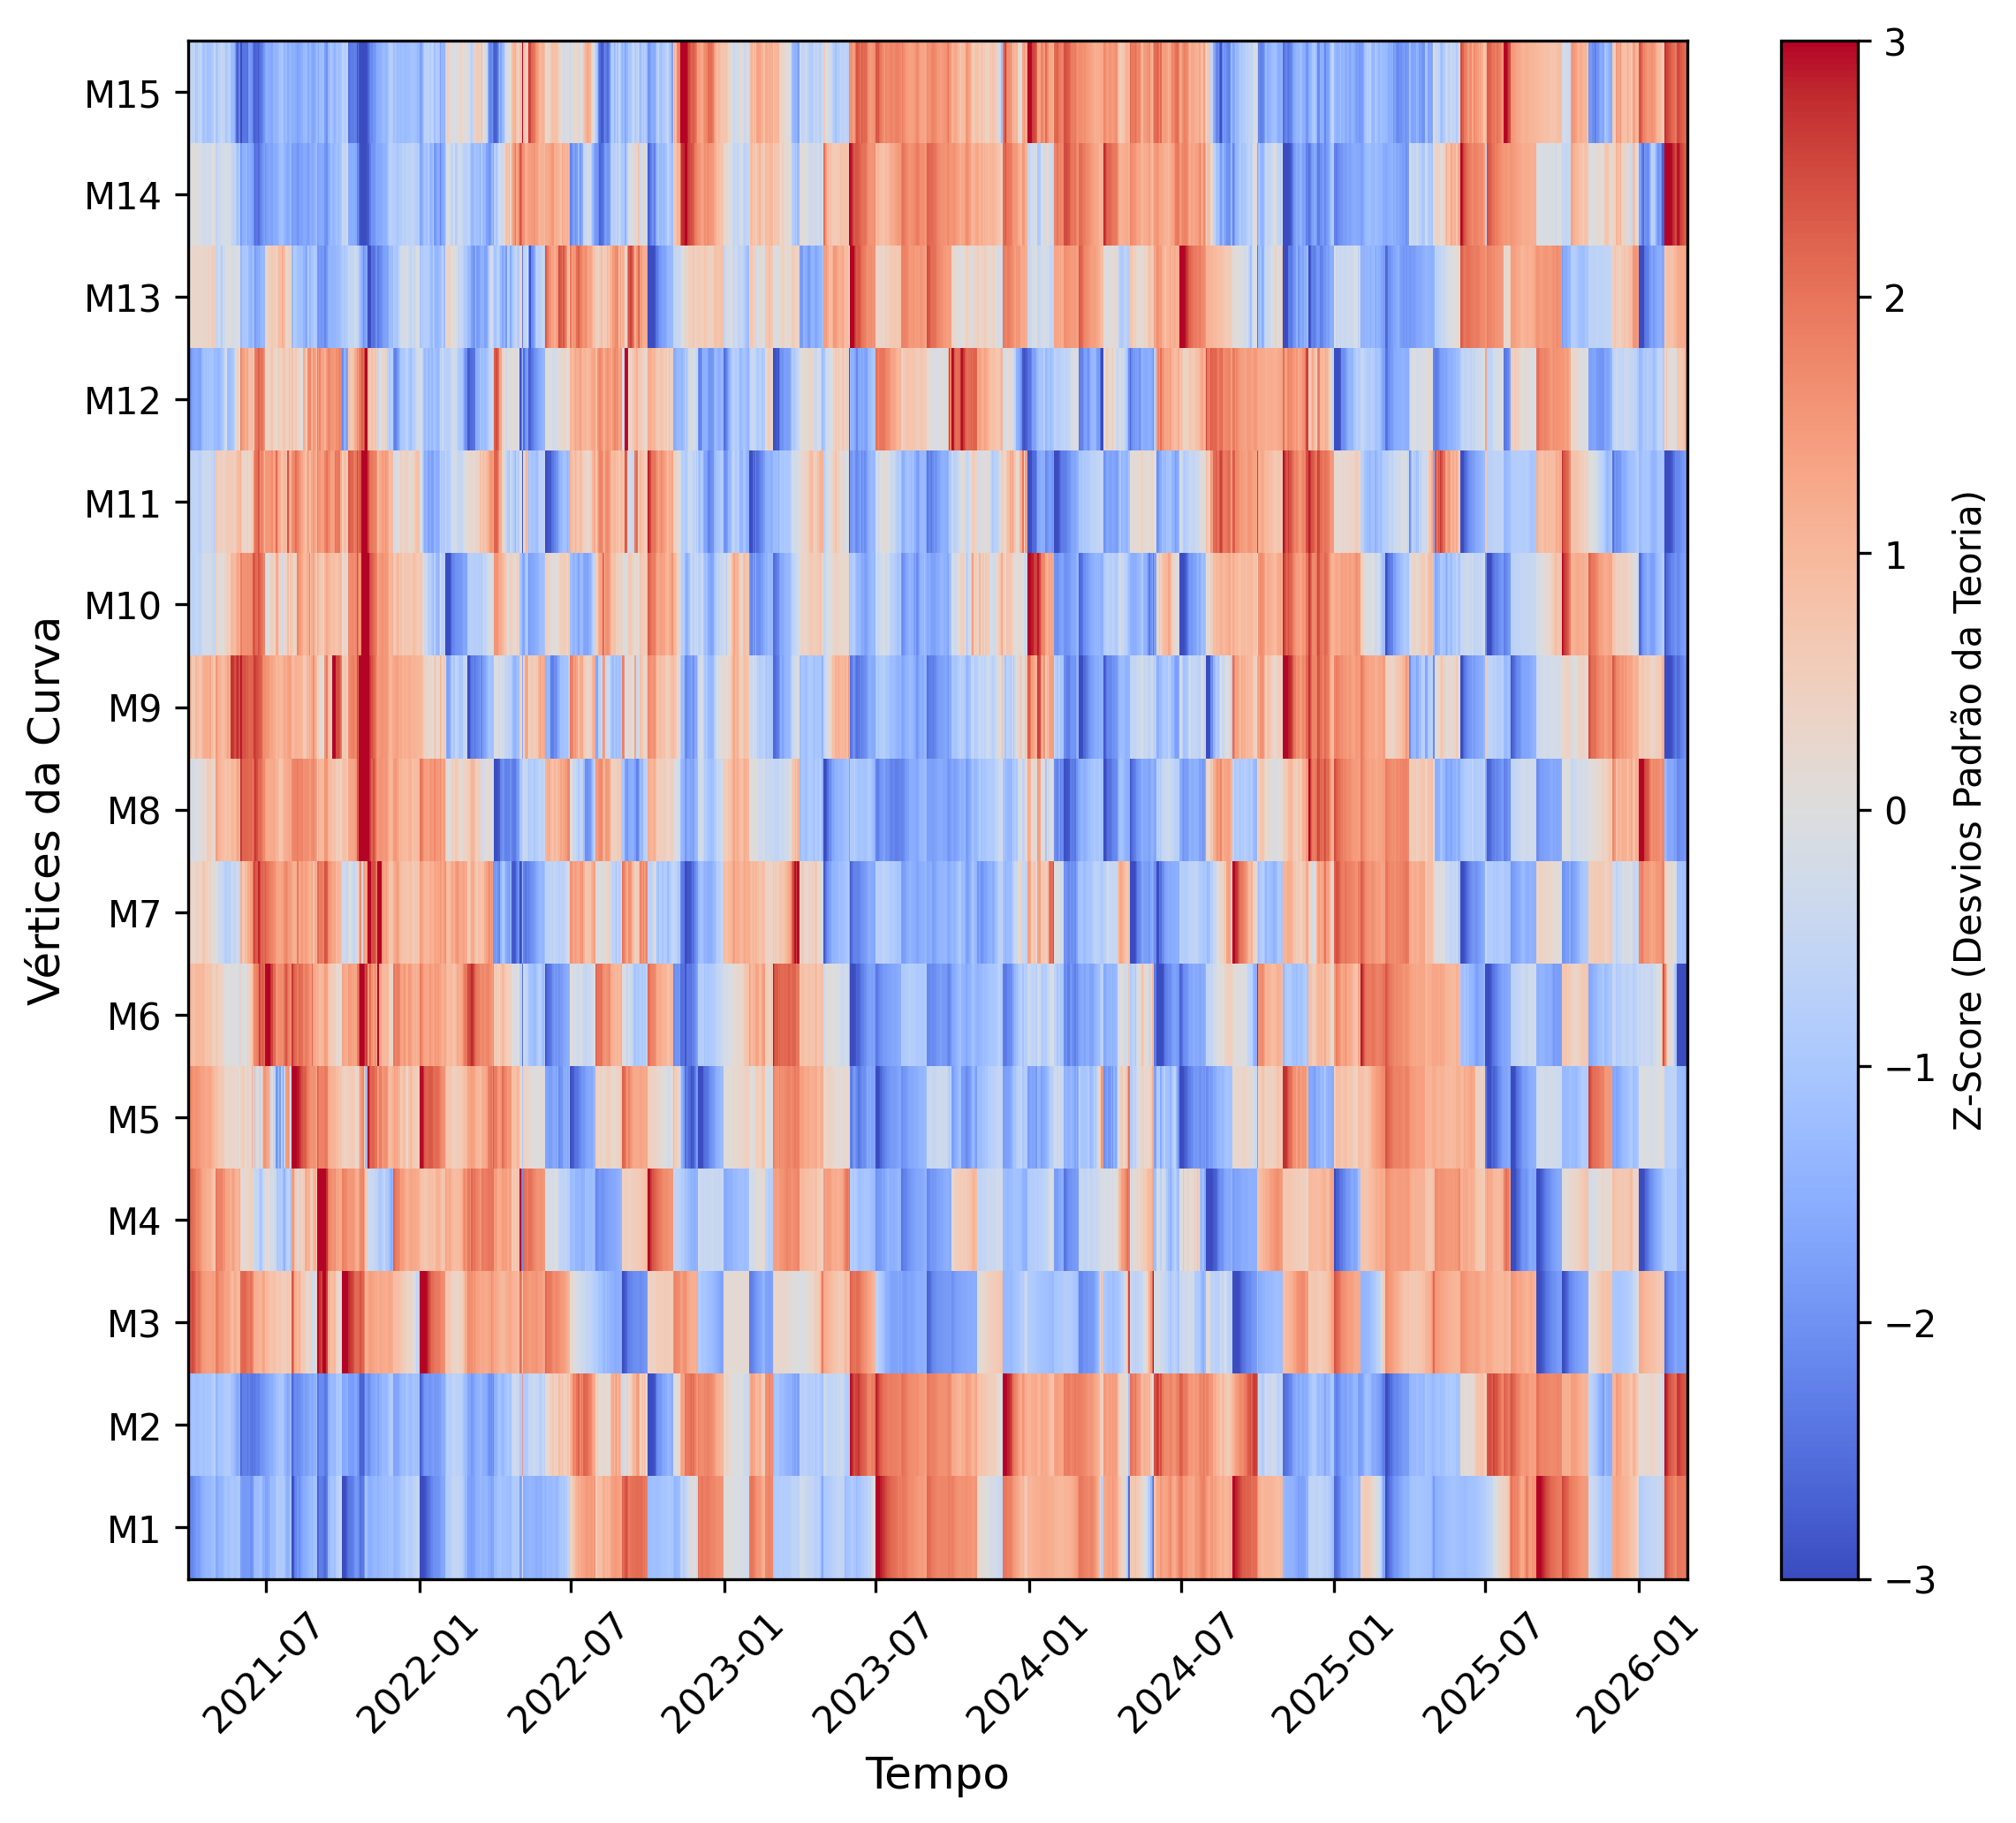
\includegraphics[width=0.78\linewidth]{media/heatmap_zscore.png}
	\caption{Heatmap do z-score dos resíduos ao longo dos vértices da curva e do tempo. Tons mais intensos indicam desvios mais extremos em relação ao padrão recente, permitindo identificar a concentração temporal e transversal das anomalias estatísticas ao longo da curva DI.}
	\label{fig:apendice_heatmap}
\end{figure}


\end{document}